\documentclass[11pt]{article}
\usepackage[margin=1in]{geometry}
\usepackage{graphicx}
\usepackage{amsmath}
\usepackage{pgfplots}
\usepackage{titlesec}
\usepackage{url}
\usepackage{verbatim}
\graphicspath{{../Screenshots/}}
\newcommand{\memoheader}[4]{
  \noindent
  \textbf{From:} #2\\ 
  \textbf{To:} #1\\
  \textbf{Date:} #3\\
  \textbf{Subject:} #4\\[1ex]\hrule\vspace{1.5ex}
}
\titleformat{\section}
  {\normalfont\Large\bfseries}   % format
  {Problem~\thesection}          % label
  {1em}                          % sep
  {}                             % before-code

\renewcommand{\thesection}{\arabic{section}}





\begin{document}
\memoheader{Prof. Gentry}
            {Miguel Cuaycong}
            {\today}
            {EMS 180 - HW5}
\section{}
Cost equation: $$Cost = C_{\text{materials}} + C_{\text{dedicated}} + C_{capital} + C_{overhead}$$
Where:
\\
$C_{\text{materials}} = C_m*\frac{m}{1-f}$
\\
$C_{\text{dedicated}} = \frac{C_t}{n}\text{ceiling}(\frac{n}{n_t})$
\\
$C_{capital} = \frac{L_f}{\dot{n}} \frac{C_c}{t_{wo}}$
\\
$C_{overhead}=\frac{\dot{C}_{oh}}{\dot{n}}$
\subsection{List each of the numbers that will be used as inputs to the cost equation. You
should provide a brief explanation of how you selected your variables from the ranges
provided in the software.}
\begin{center}
  \begin{tabular}{|c|c|c|}
    \hline
    Capital cost ($C_c$) & 180,000 dollars & Actual cost of equipment[1]
    \\
    \hline
    Material utilization factor ($1-f$) & 0.935 & Average from CES EduPack
    \\
    \hline
    Production rate ($\dot{n}$)& 0.5 hours & Average from [2]
    \\
    \hline
    Tooling cost ($C_t$)& 1500 dollars & Average from [3]
    \\
    \hline
    Tool life ($n_t$)& 5000 & Average from CES EduPack
    \\
    \hline
    Material cost ($C_m$) & 2.27 dollars/kg & Average from CES EduPack
    \\
    \hline
  \end{tabular}
\end{center}
List of references:
\begin{enumerate}
  \item Teyun's 1100Tons Al Extrusion Press Machine
  \item HOONLY website \url{https://haluminium.com/Product/analysis-on-production-process-of-6063-alloy-extruded-profiles/}
  \item Profile Precision Extrusion website \url{https://profileprecisionextrusions.com/common-questions-answered/}
\end{enumerate}


\subsection{Calculate the cost per frame if 5,000 frames are manufactured. You must show
your work or provide information on where this comes from.}
additional parameters:
\\
$m = 0.150$kg
\\
$C_{oh} = 100$ dollars/hr
\\
$t_{wo} = 5$ years
\\
$n = 5000$parts
\\
$L_f = 0.9$
$$Cost = C_m\frac{m}{1-f} + \frac{C_t}{n}\text{ceiling}(\frac{n}{n_t}) + \frac{L_f}{\dot{n}} \frac{C_c}{t_{wo}} + \frac{\dot{C}_{oh}}{\dot{n}}$$
$$Cost = 2.27\frac{0.15}{0.935} + \frac{1500}{5000}\text{ceiling}(\frac{5000}{5000}) + \frac{0.9}{0.5} \frac{180000}{5(\frac{12*4*7*24}{1})} + \frac{100}{0.5}$$
$$Cost = 208.7\text{ dollars}$$
\subsection{On log-log axes, plot the price versus batch size for the frames, spanning batch
sizes of at least 100-100,000 frames. You must use a plotting program (such as Excel or
MATLAB), NOT CES EduPack.}
\begin{center}
  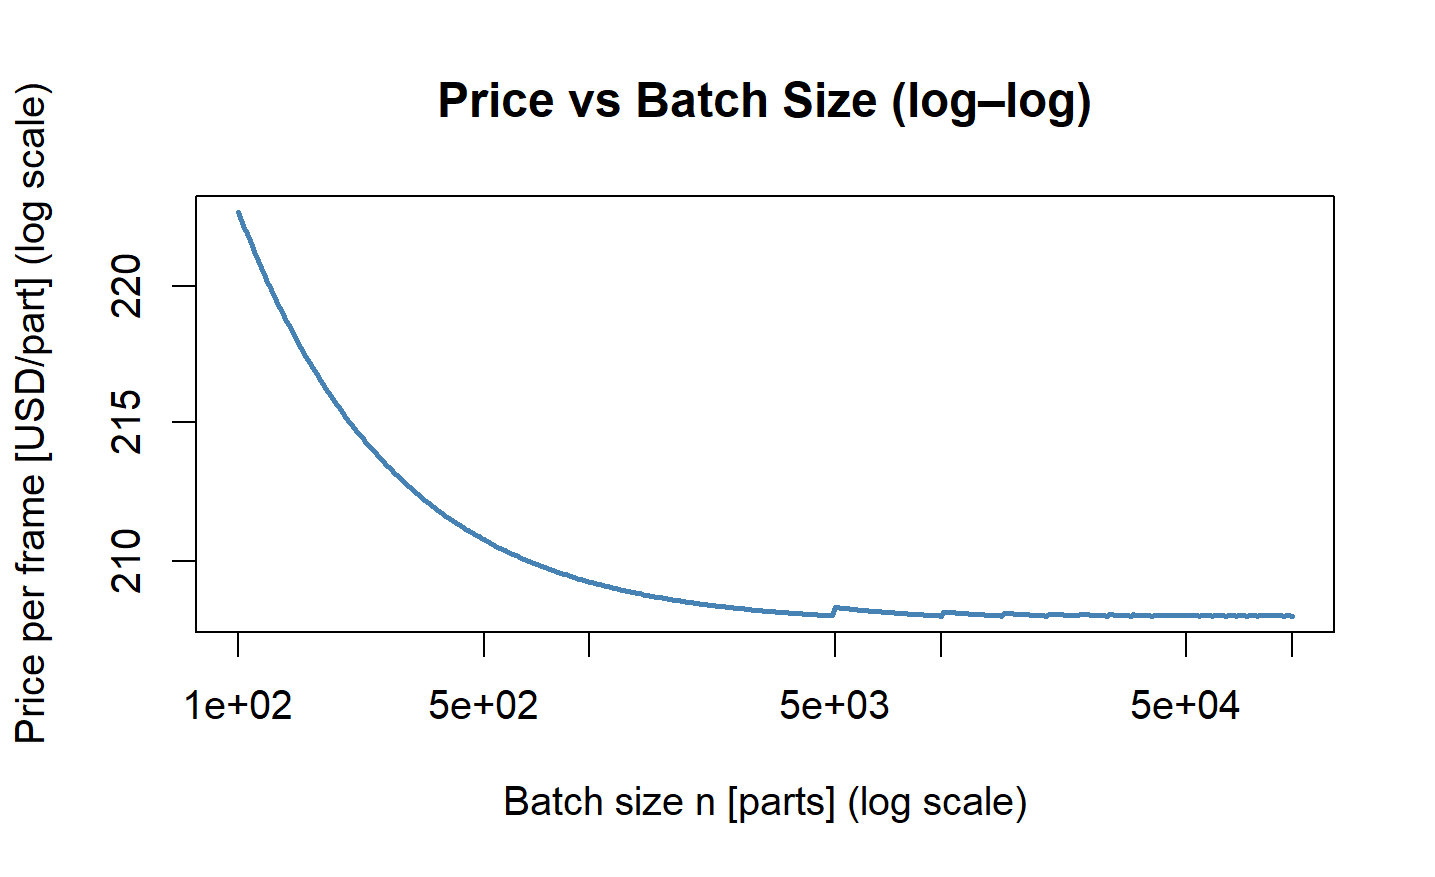
\includegraphics[width=\textwidth]{Rplot01.png}
\end{center}
$$\text{Cost} = (C_m\frac{m}{1-f}  + \frac{L_f}{\dot{n}} \frac{C_c}{t_{wo}} + \frac{\dot{C}_{oh}}{\dot{n}} )+ \frac{C_t}{n}\text{ceiling}(\frac{n}{n_t})$$
$$log(\text{Cost}) = \text{const.} + \log (\frac{C_t}{n})+\log \text{ceiling}(\frac{n}{n_t})$$
R language is used to create the plot. 
\\
Generative AI is used for plot aesthetics.
\newpage
\subsection{Code snippet used:}
\begin{verbatim}
Cm   <- 2.27
m    <- 0.150
f    <- 0.065
Ct   <- 1500
nt   <- 5000
Lf   <- 0.9
Cc   <- 180000
two_hr <- 5 * 365 * 24
Coh  <- 100
n_dot <- 0.5

cost_per_part <- function(n) {
  Cm * m / (1 - f) +
    (Ct / n) * ceiling(n / nt) +
    (Lf / n_dot) * (Cc / two_hr) +
    (Coh / n_dot)
}
## GEN AI CODE START
# Batch sizes and costs
n_vals   <- round(exp(seq(log(100), log(1e5), length.out = 400)))
price_usd <- cost_per_part(n_vals)

# Log-log plot
plot(n_vals, price_usd,
     log = "xy", type = "l", lwd = 2, col = "steelblue",
     xlab = "Batch size n [parts] (log scale)",
     ylab = "Price per frame [USD/part] (log scale)",
     main = "Price vs Batch Size (log–log)")
\end{verbatim}

\end{document}